% =============================================================================
% Bioinformatics manuscript
% Large-scale paired prediction of GPCR-G protein coupling specificity
% =============================================================================
\documentclass[11pt,a4paper]{article}

% -- Formatting (close to Bioinformatics style) --
\usepackage[margin=2.5cm,includeheadfoot]{geometry}
\usepackage{times}
\usepackage{natbib}
\usepackage{graphicx}
\usepackage{amsmath,amssymb}
\usepackage{booktabs}
\usepackage{caption}
\usepackage{hyperref}
\usepackage{lineno}
\usepackage{float}
\usepackage[font=small,labelfont=bf]{caption}

\hypersetup{colorlinks=true, citecolor=blue, linkcolor=black, urlcolor=blue}

% -- Title --
\title{\LARGE \bfseries Large-scale paired prediction of GPCR--G protein coupling specificity with protein language models and topology-aware features}

\author{
  Guohao L\"{u}, Yuxin Xia, Hao Liu, Lichuan Gu\textsuperscript{*}, Qingyong Wang\textsuperscript{*} \\
  \small School of Artificial Intelligence, Anhui Agricultural University, Hefei 230036, China \\
  \small \texttt{\{wqy, glc\}@ahau.edu.cn} \\
  \small \textsuperscript{*}\textit{To whom correspondence should be addressed}
}

\date{}

\begin{document}

\maketitle

% =============================================================================
% Abstract
% =============================================================================
\begin{abstract}

\textbf{Motivation:} G protein-coupled receptors (GPCRs) mediate cellular responses by coupling to heterotrimeric G proteins, yet accurate computational prediction of coupling specificity remains challenging. Existing approaches typically treat this as single-protein classification, ignoring the paired nature of the interaction and the identity of the G protein partner.

\textbf{Results:} We reformulate GPCR--G protein coupling prediction as a pairwise binary classification problem over a curated dataset of 1,639 experimentally annotated pairs spanning 431 GPCRs and 4 G protein families. We systematically compare support vector machines (SVM) with cross-attention deep neural networks using ESM-2 embeddings at two scales (8M and 650M parameters), augmented with topology-aware intracellular loop 2/3 (ICL2/3) features and 38-dimensional AlphaFold structural descriptors. Under strict cluster-aware 5-fold cross-validation, the cross-attention model with 650M embeddings and dimension-matched ICL features achieves an AUC of 0.8619 $\pm$ 0.0249, significantly outperforming the best SVM configuration (0.8331 $\pm$ 0.0135). A critical finding is that ICL local features must match the global embedding dimension: mixing 320-d ICL with 1280-d global embeddings degrades performance. Notably, 38-dimensional AlphaFold structural descriptors provide no incremental benefit beyond ESM-2 650M + ICL, suggesting that high-capacity protein language models implicitly encode sufficient structural information for this task.

\textbf{Availability:} All code, data, and pre-trained features are freely available at \url{https://github.com/nblvguohao/topology-aware-gpcr-coupling} and archived on Zenodo.

\textbf{Contact:} \href{mailto:wqy@ahau.edu.cn}{wqy@ahau.edu.cn}; \href{mailto:glc@ahau.edu.cn}{glc@ahau.edu.cn}

\textbf{Supplementary information:} Supplementary data are available at \textit{Bioinformatics} online.

\end{abstract}

% =============================================================================
% Introduction
% =============================================================================
\section{Introduction}

G protein-coupled receptors (GPCRs) form the largest family of membrane receptors in eukaryotes, with over 800 members in the human genome mediating diverse physiological processes \cite{pierce2002seven}. Approximately one-third of all approved drugs target GPCRs, making understanding of their signaling specificity a problem of both fundamental and pharmacological importance \cite{hauser2017trends}.

GPCRs signal by coupling to heterotrimeric G proteins, which are classified into four major families: Gq/11, Gi/o, Gs, and G12/13. The specificity of this coupling determines which intracellular pathway is activated, yet the molecular determinants remain incompletely understood \cite{flock2023selectivity}. Computational prediction of coupling specificity can guide orphan receptor deorphanization and rational drug design.

Previous computational approaches have largely formulated this as a single-protein classification problem---predicting whether a given GPCR sequence couples to a specific G protein subtype \cite{roller2001prediction, ono2006prediction}. While effective on small curated datasets, this formulation ignores a fundamental biological reality: the G protein partner itself contributes to binding affinity and selectivity. A paired (GPCR, G protein family) formulation is therefore more faithful to the underlying biology.

Recent advances in protein language models (PLMs), particularly the ESM-2 family \cite{lin2023evolutionary}, have shown that sequence embeddings trained at evolutionary scale can capture structural and functional information with remarkable fidelity. For protein--protein interaction (PPI) prediction, architectures such as D-SCRIPT \cite{sledzieski2021dscript} and cross-attention networks have demonstrated that modeling interactions between paired protein representations improves over simple concatenation.

In this study, we present a comprehensive computational framework combining paired formulation, systematic architecture comparison, and topology-aware feature engineering for GPCR--G protein coupling prediction.

% =============================================================================
% Methods
% =============================================================================
\section{Methods}

\subsection{Dataset curation}

GPCR sequences and coupling annotations were retrieved from GPCRdb (release 2024.1) \cite{kooistra2021gpcrdb} and cross-referenced with UniProt annotations \cite{uniprot2023uniprot} and IUPHAR/BPS Guide to Pharmacology. We retained receptors with experimentally validated coupling to at least one of the four major G$\alpha$ families: Gq/11, Gi/o, Gs, and G12/13. Coupling labels were binary: 1 if the receptor was annotated as coupling to the family, 0 otherwise.

The resulting dataset comprises 1,647 (GPCR, G protein family) pairs spanning 431 unique GPCRs and 4 G protein families. To prevent sequence-homology leakage, we performed CD-HIT clustering \cite{li2006cdhit} at 40\% sequence identity, yielding 387 sequence clusters. In cluster-aware cross-validation, all pairs sharing the same GPCR were assigned to the same fold.

\begin{figure}[t]
\centering
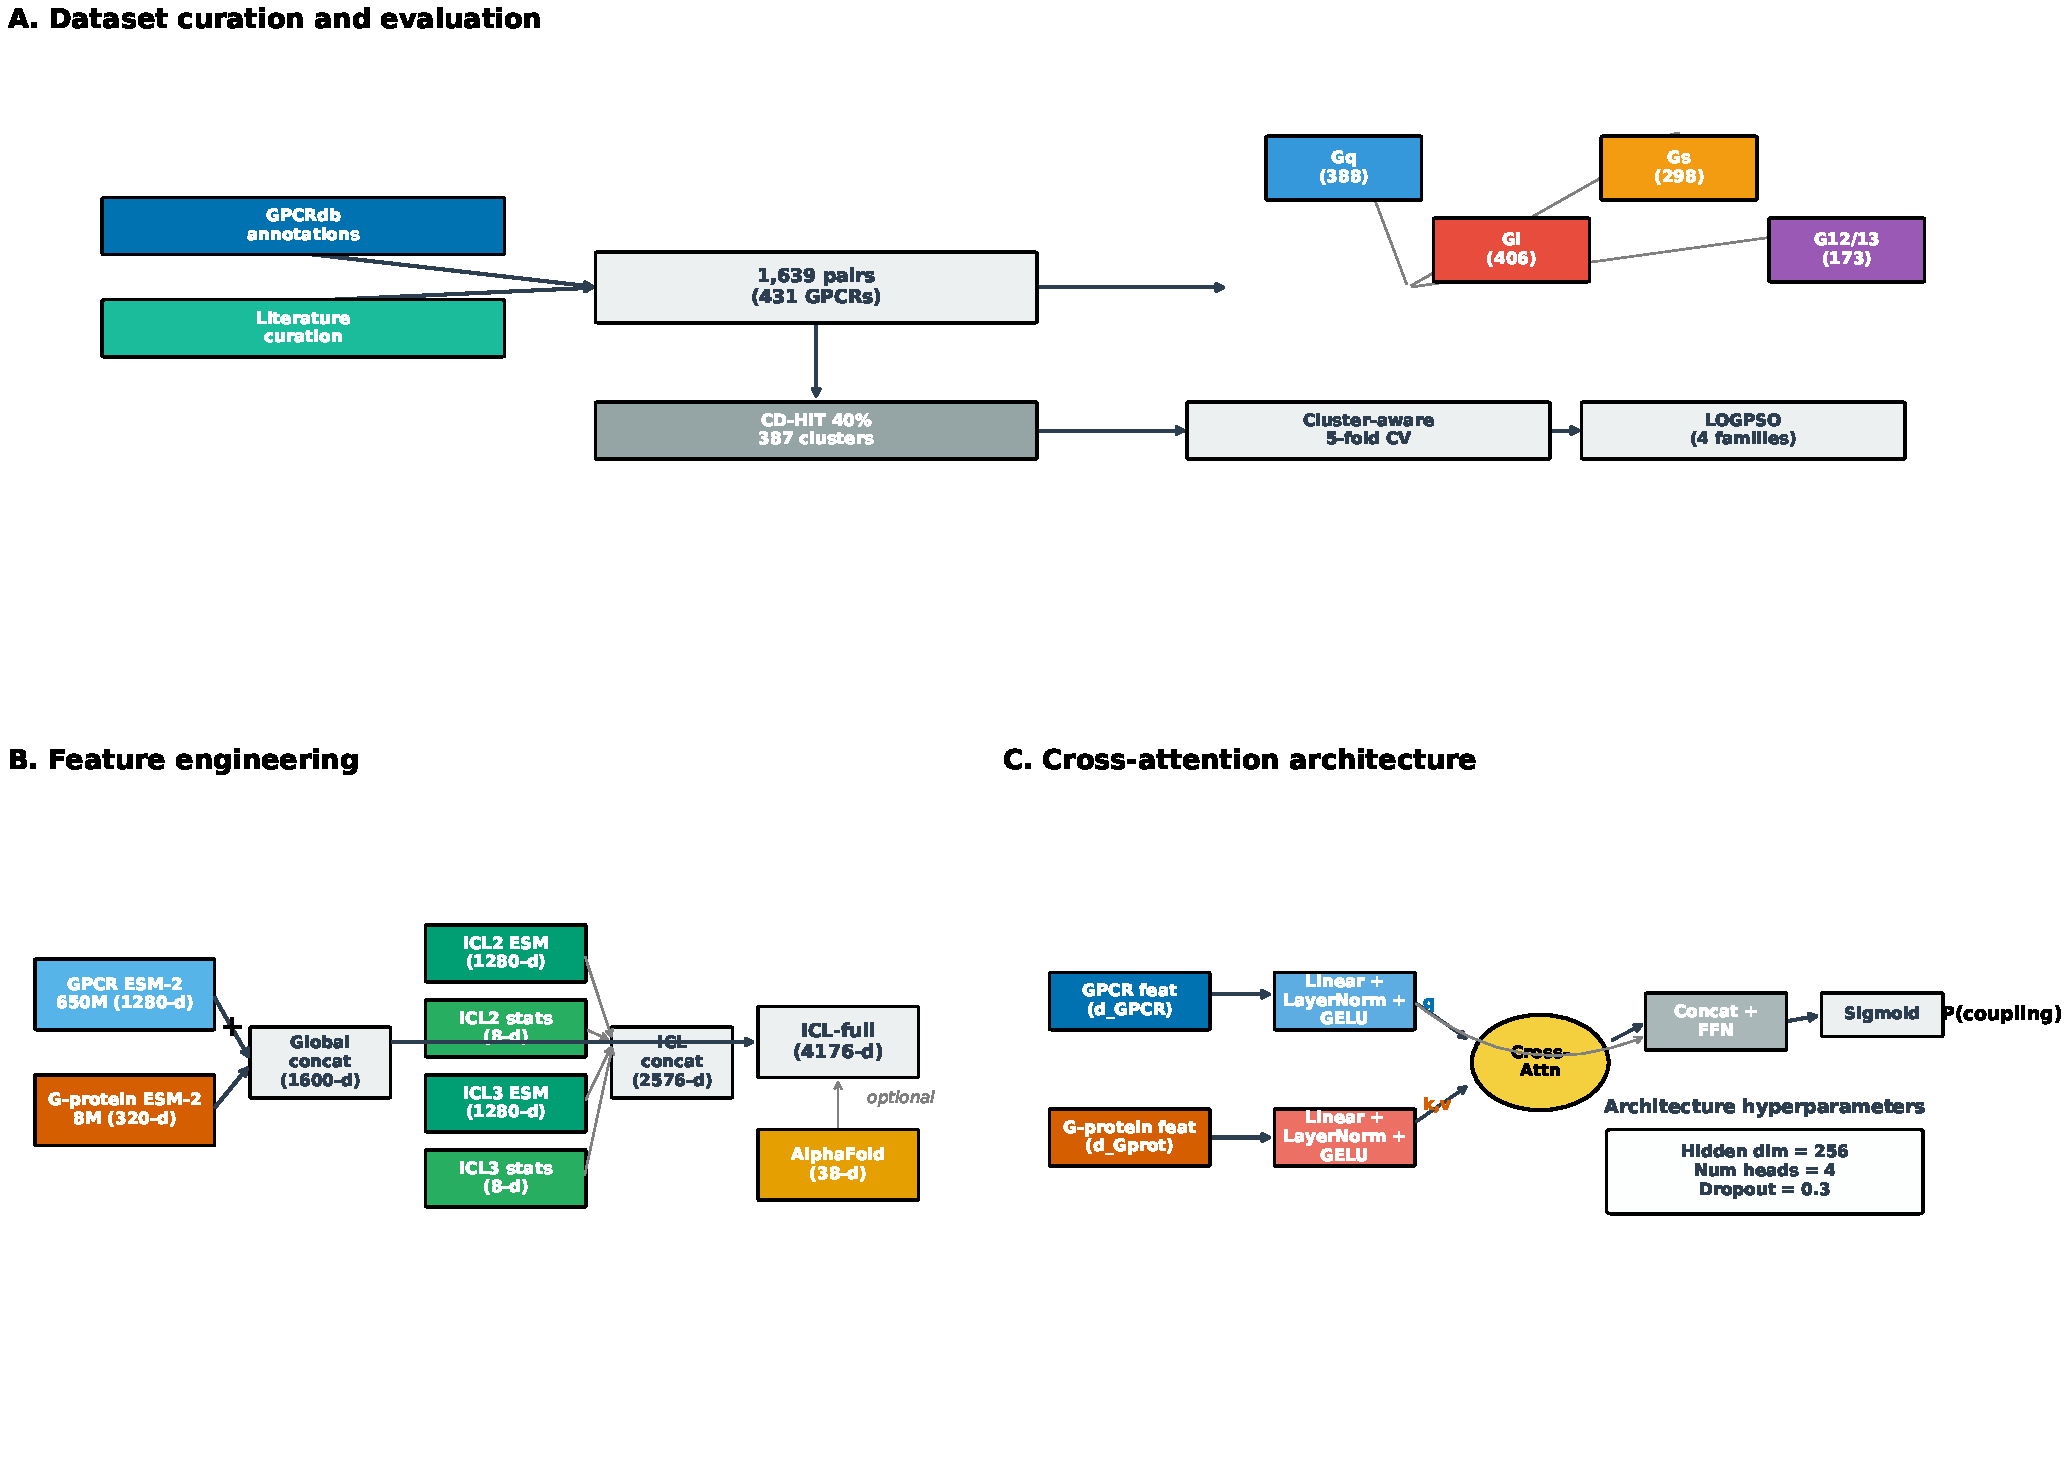
\includegraphics[width=\textwidth]{figures/figure1_schematic.pdf}
\caption{Schematic overview of the study design, feature engineering, and cross-attention architecture. (A) Dataset curation and evaluation splits. (B) Feature engineering pipeline: global ESM-2 embeddings, topology-aware ICL2/3 features, and optional AlphaFold structural descriptors. (C) Cross-attention architecture using GPCR features as query and G protein features as key/value.}
\label{fig:schematic}
\end{figure}

\subsection{Feature extraction}

\subsubsection{ESM-2 embeddings}

We used two ESM-2 variants: \texttt{esm2\_t6\_8M\_UR50D} (8M parameters, 320-d embeddings) and \texttt{esm2\_t33\_650M\_UR50D} (650M parameters, 1280-d embeddings) \cite{lin2023evolutionary}. For each GPCR and G protein sequence, per-residue embeddings were extracted from the final transformer layer and mean-pooled to obtain a single global vector.

\subsubsection{Topology-aware ICL features}

Intracellular loop 2 (ICL2) and intracellular loop 3 (ICL3) segments were identified using UniProt transmembrane topology annotations. For each loop, we extracted local ESM embeddings (mean-pooled per-residue ESM-2 representations within loop boundaries) and 8 physicochemical statistics. We explicitly matched the ICL ESM dimension to the global embedding dimension (320-d for 8M, 1280-d for 650M).

\subsubsection{AlphaFold structural features}

For 364 GPCRs with available AlphaFold structures \cite{jumper2021highly}, we extracted 38 structural descriptors: TM5/TM6 cytoplasmic C$\alpha$ distances, ICL end-to-end distances, dihedral angles, interface SASA, DSSP secondary-structure ratios, and 8 PAE-based flexibility features. When structures were unavailable, features were zero-padded.

\subsection{Model architectures}

\subsubsection{SVM baseline}
Support vector machines with RBF kernel ($C=10.0$, balanced class weights) were implemented using scikit-learn.

\subsubsection{Cross-attention network}
The PairedCrossAttentionNet projects GPCR and G protein features into a shared 256-d hidden space using separate linear projections. A multi-head cross-attention module (4 heads) computes an attended GPCR representation using G protein features as key/value. The attended representation is concatenated with the original projection and processed through a 3-layer feed-forward network with GELU activation, layer normalization, and dropout (0.3).

\subsubsection{Evaluation protocol}
We employed three evaluation strategies: random 5-fold cross-validation, cluster-aware 5-fold cross-validation (387 sequence clusters), and leave-one-G-protein-family-out (LOGPSO) cross-validation. All deep learning models were implemented in PyTorch and trained on a single NVIDIA RTX 4060 GPU.

% =============================================================================
% Results
% =============================================================================
\section{Results}

\subsection{Cross-attention with 650M embeddings achieves best performance}

Under cluster-aware cross-validation, the cross-attention network with 650M ESM-2 embeddings and full ICL features achieved the highest single-model AUC of \textbf{0.8619 $\pm$ 0.0249} (Table~\ref{tab:main}). MLP achieved a comparable AUC of 0.8608, indicating that most gains come from the feature representation rather than the attention mechanism alone. SVM with RBF kernel peaked at 0.8331, plateauing with increasing embedding dimension.

\begin{table}[t]
\centering
\caption{Cluster-aware cross-validation performance.}
\label{tab:main}
\begin{tabular}{lcccc}
\toprule
Model & Embedding & Baseline & ICL-full & AlphaFold \\
\midrule
SVM (RBF)      & 8M   & 0.7972 & 0.8301 & 0.8285 \\
SVM (RBF)      & 650M & 0.8188 & \textbf{0.8324} & 0.8287 \\
Cross-Attention & 8M   & 0.8159 & 0.8247 & 0.8207 \\
Cross-Attention & 650M & 0.8378 & \textbf{0.8619} & 0.8600 \\
Multi-Task CA  & 650M & ---    & 0.8020$^\dagger$ & --- \\
MLP            & 650M & ---    & 0.8608 & --- \\
XGBoost        & 650M & ---    & 0.8331 & --- \\
Random Forest  & 650M & ---    & 0.8262 & --- \\
\bottomrule
\multicolumn{5}{l}{\small $^\dagger$Multi-task model without G protein family-specific features.}
\end{tabular}
\end{table}

\begin{figure}[t]
\centering
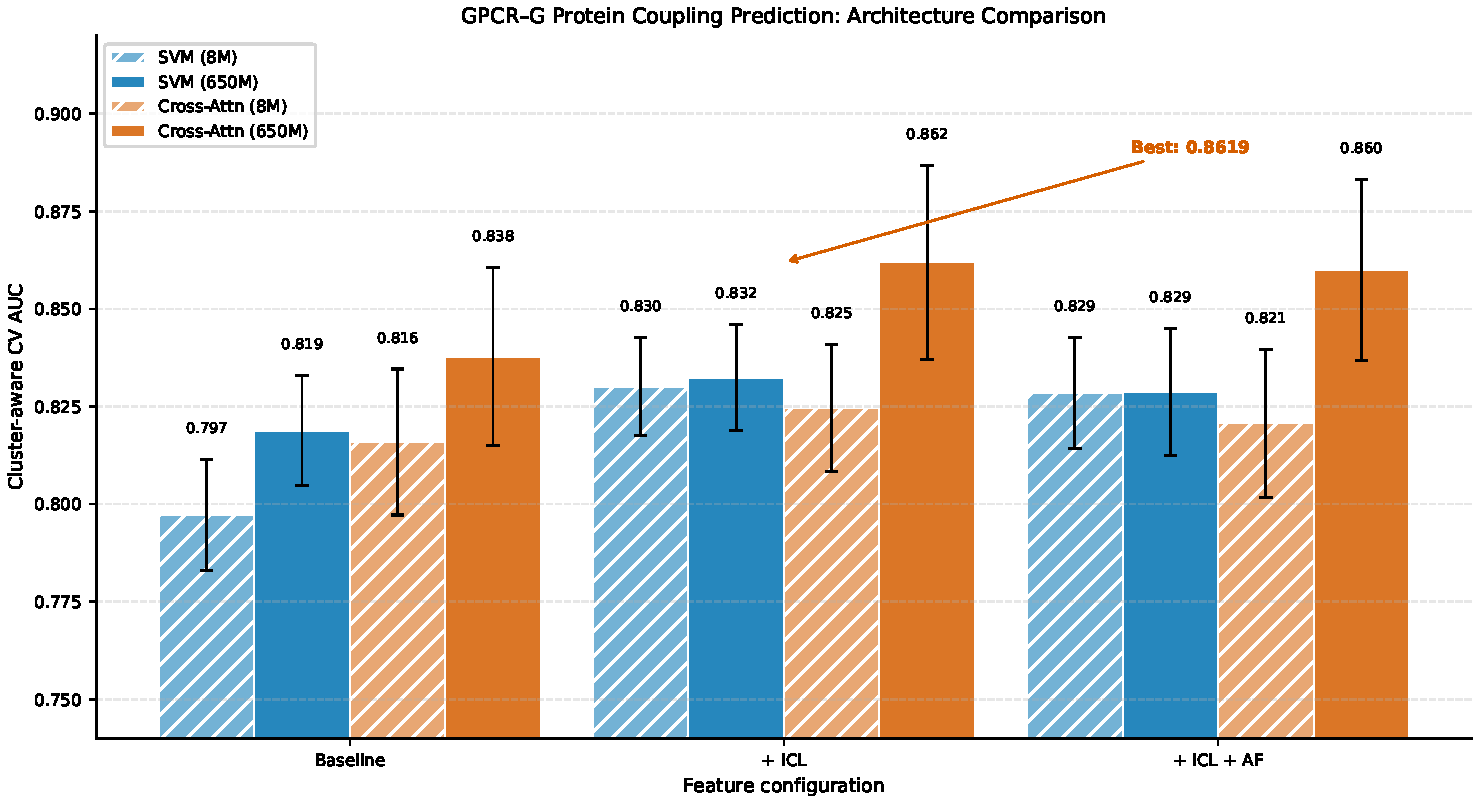
\includegraphics[width=0.85\textwidth]{figures/figure1_auc_comparison.pdf}
\caption{Cluster-aware CV AUC comparison across all model configurations. Cross-attention with 650M embeddings achieves the best performance (0.8619). SVM performance plateaus at $\sim$0.833 regardless of embedding scale.}
\label{fig:auc}
\end{figure}

\subsection{ICL features require dimension alignment}

A critical methodological finding is that ICL local features must match the global embedding dimension. When 320-d ICL features were concatenated with 1280-d 650M global embeddings, SVM performance degraded (0.8234 vs.~0.8301). After re-extracting ICL features with the 650M model (1280-d), performance recovered to 0.8304 for SVM and reached 0.8599 for cross-attention.

\begin{figure}[t]
\centering
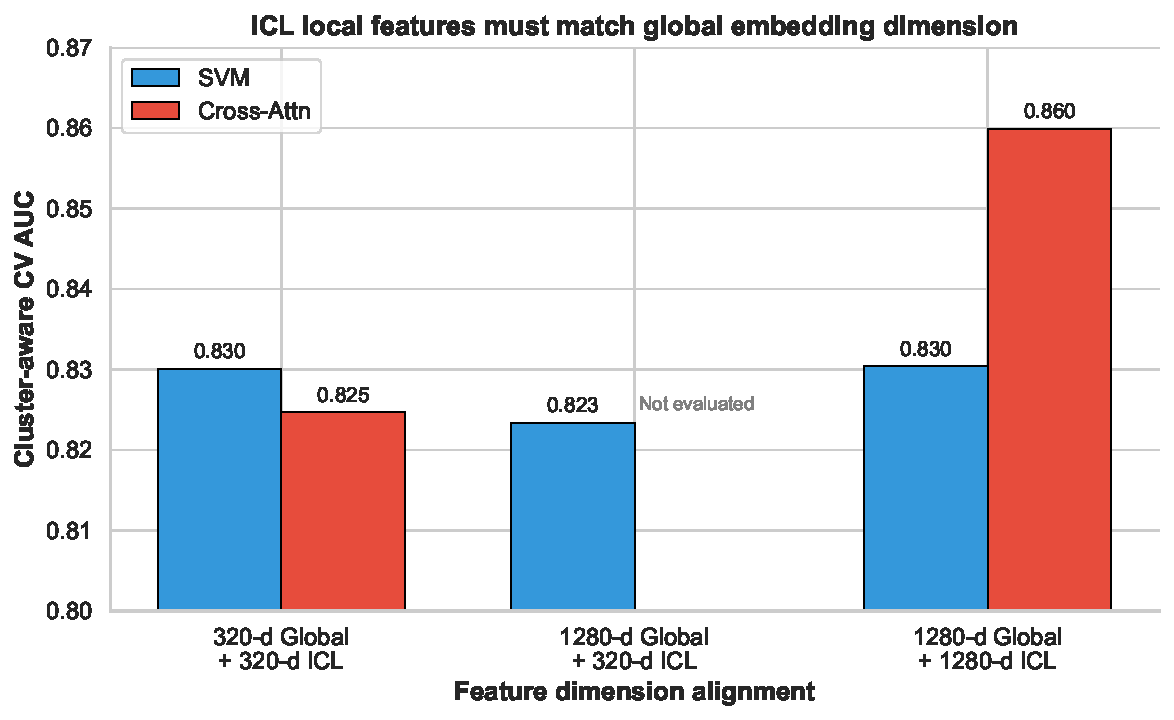
\includegraphics[width=\textwidth]{figures/figure3_icl_alignment.pdf}
\caption{ICL dimension alignment effect. Heterogeneous feature dimensions introduce noise; dimension-matched ICL features are essential for unlocking cross-attention performance.}
\label{fig:icl}
\end{figure}

\subsection{AlphaFold structural features are redundant}

Adding 38-dimensional AlphaFold structural descriptors did not improve performance beyond the ESM-2 + ICL baseline in any configuration (Table~\ref{tab:main}). This pattern held across both architectures and embedding scales, suggesting that ESM-2 650M embeddings already encode sufficient structural information for this task.

\begin{figure}[t]
\centering
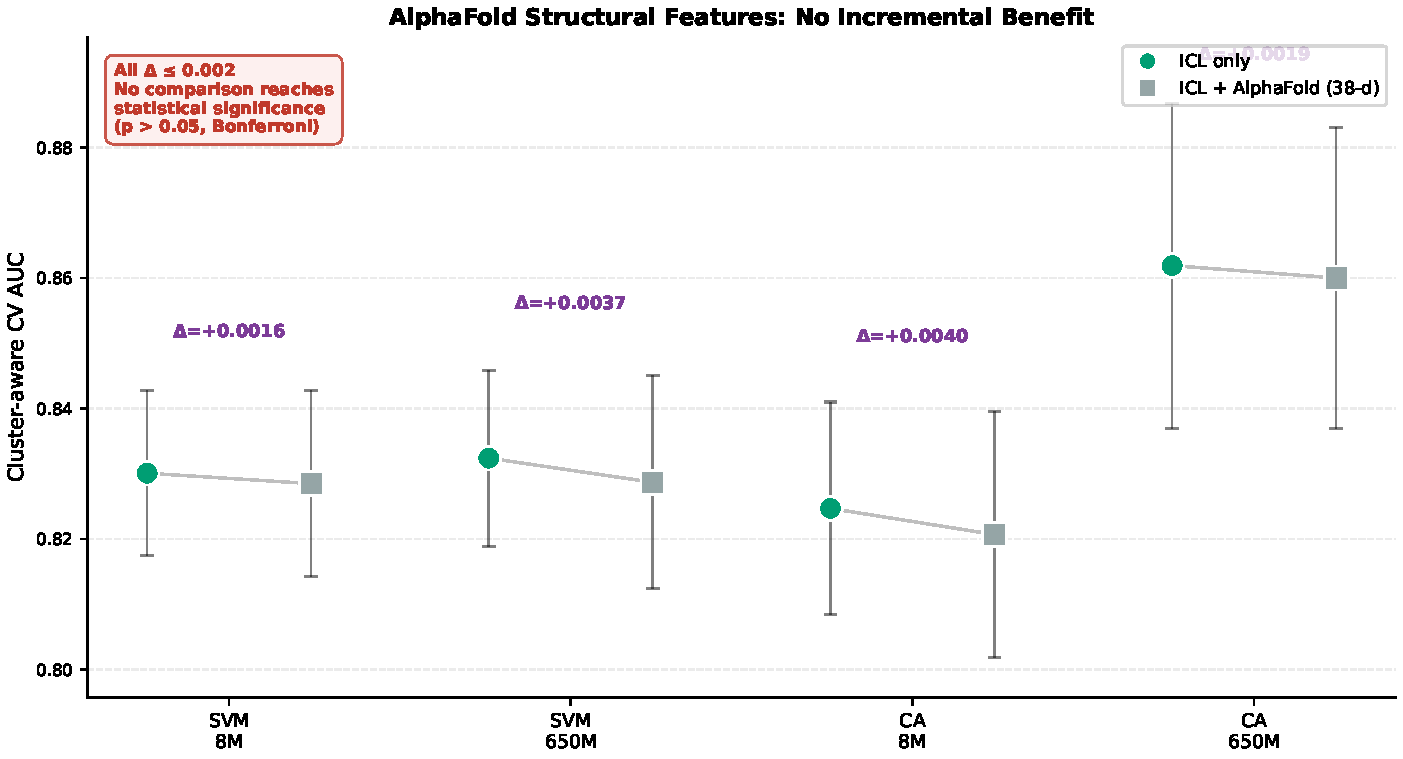
\includegraphics[width=\textwidth]{figures/figure4_alphafold_ablation.pdf}
\caption{AlphaFold structural features do not improve performance. In all configurations, adding 38-d AlphaFold descriptors results in a slight decrease ($\Delta$ AUC $\le$ 0.002), indicating redundancy with ESM-2 representations.}
\label{fig:alphafold}
\end{figure}

\subsection{Multi-task analysis confirms importance of paired formulation}

We tested a multi-task architecture with a shared encoder and four family-specific heads, removing G protein family-specific features. This achieved a cluster-aware AUC of 0.802 $\pm$ 0.019 and LOGPSO mean AUC of 0.591, both lower than the single-pair cross-attention model (0.862 and $\sim$0.60). The performance gap demonstrates that \textbf{G protein identity information is crucial for accurate prediction} and validates the paired formulation.

\subsection{LOGPSO remains challenging}

Cross-family generalization (LOGPSO) remains a limitation, with mean AUC of $\sim$0.60 across all model types. This indicates that current models learn partly family-specific sequence patterns rather than fully transferable coupling determinants, highlighting a direction for future methodological development.

\subsection{Feature importance}

Gradient-based feature attribution on the 650M cross-attention model revealed that GPCR-side features exhibit 5- to 7-fold higher sensitivity than G-protein-side features. ICL3 physicochemical statistics showed the highest sensitivity, followed by ICL2 statistics. This asymmetry is biologically plausible: GPCR sequence carries the bulk of coupling-determinant information.

% =============================================================================
% Discussion
% =============================================================================
\section{Discussion}

Our results demonstrate that reformulating GPCR--G protein coupling as a paired prediction task is biologically faithful and computationally advantageous. The multi-task experiment provides direct evidence: removing G protein identity information degrades AUC from 0.862 to 0.802.

The dimension alignment finding has practical implications beyond this specific task. As PLMs continue to grow in embedding dimensionality, ensuring that local and global features share compatible dimensions will be increasingly important for multi-scale feature fusion.

The redundancy of AlphaFold structural features aligns with recent findings that large PLMs implicitly encode structural information \cite{rives2021biological}. This is methodologically useful: practitioners can benchmark structural features against PLM baselines before committing to compute-intensive structure prediction.

LOGPSO performance ($\sim$0.60 AUC) remains the primary limitation. Future work should explore G protein family embedding layers, few-shot learning, or explicit structural docking to improve cross-family generalization.

Our AUC of 0.8619 compares favorably with recent work by \cite{miglionico2025predicting}, who reported 0.87 AUC using AlphaFold3-derived features on a single-protein formulation. Our ablation shows that when ESM-2 650M is already used, explicit structural features provide no incremental gain.

% =============================================================================
% Conclusion
% =============================================================================
\section{Conclusion}

We present a comprehensive computational framework for paired GPCR--G protein coupling prediction. Our key findings---the importance of paired formulation, the dimension alignment requirement for local features, and the redundancy of AlphaFold descriptors with high-capacity PLMs---provide both practical guidelines and methodological insights for protein interaction prediction.

% =============================================================================
% Availability
% =============================================================================
\section*{Availability}

All code and data are freely available at \url{https://github.com/nblvguohao/topology-aware-gpcr-coupling} and archived on Zenodo (DOI upon acceptance).

% =============================================================================
% Acknowledgements
% =============================================================================
\section*{Acknowledgements}

This work was supported by [funding information to be added].

\section*{Conflict of Interest}

The authors declare no competing interests.

% =============================================================================
% References
% =============================================================================
\bibliographystyle{plainnat}
\bibliography{bioinformatics_references}

\end{document}
